\documentclass[11pt]{article}

% ============================================================
% PACKAGES
% ============================================================

\usepackage[margin=1in]{geometry}
\usepackage{amsmath,amssymb}
\usepackage{array}
\usepackage{booktabs}
\usepackage{tabularx}
\usepackage{enumitem}
\usepackage{microtype}
\usepackage[most]{tcolorbox}
\usepackage{tikz}
\usepackage{hyperref}

% ============================================================
% FORMATTING
% ============================================================

\setlength{\parindent}{0pt}
\setlength{\parskip}{0.65em}

\setlist[itemize]{itemsep=0.3em, topsep=0.4em}
\setlist[enumerate]{itemsep=0.3em, topsep=0.4em}

\hypersetup{
    colorlinks=false,
    pdfborder={0 0 0}
}

% ============================================================
% WHITEBOARD ENVIRONMENT
% ============================================================

\newtcolorbox{whiteboard}{
    enhanced,
    breakable,
    colback=white,
    colframe=black,
    boxrule=0.9pt,
    sharp corners,
    title=\textbf{WHITEBOARD},
    fonttitle=\bfseries,
    attach boxed title to top left={
        xshift=0.4cm,
        yshift=-2mm
    },
    boxed title style={
        colback=white,
        colframe=black,
        sharp corners
    },
    before skip=1em,
    after skip=1em
}

\newcommand{\boardtakeaway}[1]{
    \begin{center}
    \fbox{
        \parbox{0.88\linewidth}{
            \centering
            \textbf{#1}
        }
    }
    \end{center}
}

% ============================================================
% DOCUMENT
% ============================================================

\begin{document}

\begin{center}
    {\LARGE \textbf{Aristotle's Organon}}\\[0.4em]
    {\large From Dialectical Practice to Systematic Formal Logic}\\[0.8em]
    \textit{History of Logic}\\[0.5em]
    \textbf{Primary source:} William and Martha Kneale,
    \textit{The Development of Logic}, Chapter II,
    ``Aristotle's Organon.''
\end{center}

\vspace{1em}

% ============================================================
% INTRODUCTION
% ============================================================

\section{Aristotle and the Systematization of Logic}

In the preceding lecture, we saw that substantial reflection on
valid inference existed before Aristotle.

Greek geometers had developed the ideal of demonstration.
Zeno and Socrates had used refutation through consequences.
Sophists and Megarians had raised problems concerning valid and
invalid argument.
Plato had investigated truth, necessary connexion, definition,
negation, and predication.

What had not yet appeared was a systematic formal theory tying
such logical discoveries together.

Aristotle's decisive contribution is therefore best understood as
\textbf{systematization}.

\begin{whiteboard}
\textbf{FROM PRE-ARISTOTELIAN LOGIC TO ARISTOTLE}

\[
\begin{array}{c}
\text{demonstration}\\
\text{dialectic}\\
\text{fallacy}\\
\text{logical principles}\\
\downarrow\\
\boxed{\text{SYSTEMATIC FORMAL THEORY}}
\end{array}
\]

\[
\boxed{\text{Aristotle's decisive achievement: SYSTEMATIZATION}}
\]
\end{whiteboard}

The achievement is enormous, but the Kneales also emphasize an
important qualification.

The framework Aristotle systematizes is centered upon
\textbf{general subject--predicate propositions}. That choice
makes his theory extraordinarily powerful in one domain while
also narrowing the kinds of logical form he develops.

Our task is therefore to understand both:

\begin{enumerate}
    \item what Aristotle discovered; and
    \item what the structure of his system caused him to overlook.
\end{enumerate}

% ============================================================
% PART I
% ============================================================

\part*{I. From Dialectic to Logical Theory}

% ============================================================
\section{What Is the Organon?}
% ============================================================

The name \textit{Organon} means roughly ``instrument.''

It was not Aristotle's title for a single book written according
to one unified plan. After Aristotle's death, a number of his
works concerned with reasoning were grouped together, and the
collection eventually came to be known as the \textit{Organon}.

The modern word ``logic'' was not yet Aristotle's name for the
discipline. Nevertheless, the later conception of logic was deeply
shaped by the works included in this collection.

The principal works relevant to our discussion are:

\begin{itemize}
    \item the \textit{Categories};
    \item the \textit{Topics};
    \item the \textit{De Sophisticis Elenchis};
    \item the \textit{De Interpretatione};
    \item the \textit{Prior Analytics};
    \item the \textit{Posterior Analytics}.
\end{itemize}

\begin{whiteboard}
\textbf{ARISTOTLE'S ORGANON}

\[
\begin{array}{rcl}
\textit{Categories}
&\rightarrow&
\text{kinds / predication}
\\[0.4em]
\textit{Topics}
&\rightarrow&
\text{dialectical argument}
\\[0.4em]
\textit{Sophistical Refutations}
&\rightarrow&
\text{fallacious argument}
\\[0.4em]
\textit{De Interpretatione}
&\rightarrow&
\text{statements / opposition}
\\[0.4em]
\textit{Prior Analytics}
&\rightarrow&
\text{syllogistic form}
\\[0.4em]
\textit{Posterior Analytics}
&\rightarrow&
\text{demonstration / science}
\end{array}
\]

\boardtakeaway{The Organon is a collection, not one work written to a single plan.}
\end{whiteboard}

The chronology of Aristotle's works is difficult to determine.
Many appear to have originated as lecture materials and may have
been revised repeatedly.

For our purposes, however, a conceptual development is more
important than exact chronology.

% ============================================================
\section{A Development Within the Organon}
% ============================================================

The works reveal a movement from practical concern with debate
toward increasingly abstract reflection on logical form.

The \textit{Topics} is still closely connected with dialectical
contests.

The \textit{De Interpretatione} isolates forms and oppositions of
statements.

The \textit{Prior Analytics} develops the systematic formal theory
of syllogistic inference.

The \textit{Posterior Analytics} considers the special conditions
required for scientific demonstration.

\begin{whiteboard}
\textbf{DEVELOPMENT}

\[
\begin{array}{c}
\text{dialectical practice}\\
\downarrow\\
\text{forms of statement}\\
\downarrow\\
\text{forms of inference}\\
\downarrow\\
\text{demonstrative science}
\end{array}
\]
\end{whiteboard}

This gives us the central historical movement of the chapter:

\begin{center}
\emph{Aristotle moves from studying how people argue to studying
the forms that make arguments necessary.}
\end{center}

% ============================================================
\section{The Categories}
% ============================================================

The \textit{Categories} is difficult to classify as a work of logic
in the modern sense.

Much of it appears metaphysical. Nevertheless, its influence on
later logic was enormous.

Aristotle presents ten highest categories:

\begin{enumerate}
    \item substance,
    \item quantity,
    \item quality,
    \item relation,
    \item place,
    \item time,
    \item situation,
    \item state,
    \item action,
    \item passion.
\end{enumerate}

These are intended as extremely general kinds under which things
signified by simple expressions can fall.

\begin{whiteboard}
\textbf{THE TEN CATEGORIES}

\[
\begin{array}{ll}
\text{Substance} & \text{Relation}\\
\text{Quantity} & \text{Place}\\
\text{Quality} & \text{Time}\\
\text{Situation} & \text{State}\\
\text{Action} & \text{Passion}
\end{array}
\]

\[
\text{Categories classify kinds of being / what terms signify.}
\]
\end{whiteboard}

We will not analyze each category separately. The most important
for the history of Aristotle's logic is \textbf{substance}.

% ============================================================
\section{Primary and Secondary Substance}
% ============================================================

Aristotle distinguishes two kinds of substance.

A \textbf{primary substance} is an individual thing, such as an
individual man or horse.

A \textbf{secondary substance} is the species or genus under
which such an individual falls.

Thus we can represent the hierarchy:

\[
\text{Socrates}
\rightarrow
\text{man}
\rightarrow
\text{animal}.
\]

Socrates is an individual primary substance.

Man is a species.

Animal is a genus.

\begin{whiteboard}
\textbf{SUBSTANCE}

\[
\begin{array}{ll}
\textbf{Primary substance:}
& \text{individual}\\
& \text{e.g. Socrates, this horse}
\\[0.8em]
\textbf{Secondary substance:}
& \text{species / genus}\\
& \text{e.g. man, animal}
\end{array}
\]

\[
\text{Socrates}
\rightarrow
\text{man}
\rightarrow
\text{animal}
\]

\boardtakeaway{Primary substance is the ultimate subject.}
\end{whiteboard}

The doctrine matters logically because Aristotle treats primary
substances as the basic subjects upon which other things depend.

% ============================================================
\section{Words or Things?}
% ============================================================

The \textit{Categories} contains a basic ambiguity.

Is Aristotle classifying linguistic expressions, or the things
those expressions signify?

His terminology can suggest either answer.

The Kneales argue that Aristotle's fundamental interest is in
\textbf{types of being}, but that he uses the behavior of
linguistic expressions as evidence for distinctions among those
types.

A difficulty is that Greek did not always provide the convenient
distinctions that later logical writing developed.

We can easily distinguish:

\[
\text{man},
\qquad
\text{``man''},
\qquad
\text{humanity}.
\]

These correspond roughly to a thing or kind, a word, and an
abstract character.

Such distinctions were not always clearly marked in Aristotle's
language.

\begin{whiteboard}
\textbf{WORD / THING / PROPERTY}

\[
\begin{array}{rcl}
\text{``man''} & = & \text{word}\\
\text{man} & = & \text{kind}\\
\text{humanity} & = & \text{abstract character}
\end{array}
\]

\vspace{0.4em}

\[
\text{language}
\longrightarrow
\text{clue to types of being}
\]

\boardtakeaway{word $\neq$ thing $\neq$ property}
\end{whiteboard}

The distinction will return repeatedly in the history of logic.

% ============================================================
\section{Three Logical Consequences of the Categories}
% ============================================================

The Kneales identify three especially important consequences of
the theory of categories for later logic.

\subsection{The Dominance of Subject--Predicate Form}

If primary substance is the ultimate subject, then the basic form
of truth naturally appears to be:

\[
\text{This thing is such-and-such.}
\]

Logic therefore becomes strongly centered upon
subject--predicate propositions.

\begin{whiteboard}
\textbf{1. SUBJECT--PREDICATE DOMINANCE}

\[
\boxed{\text{Subject is Predicate}}
\]

Basic picture:

\[
\text{individual subject}
+
\text{attribute}
\]
\end{whiteboard}

This concentration eventually makes it harder to give adequate
treatment to relations and propositions involving several
independent quantifiers.

\subsection{The Singular--General Distinction Is Blurred}

Consider:

\[
\text{Socrates is a man}
\]

and

\[
\text{Man is an animal}.
\]

The first has an individual subject.

The second has a general term as subject.

Yet both can be treated within Aristotle's theory as
subject--predicate propositions involving substance.

\begin{whiteboard}
\textbf{2. SINGULAR / GENERAL}

\[
\text{Socrates is a man}
\]

\[
\text{Man is an animal}
\]

\[
\boxed{\text{These are logically different kinds of statement.}}
\]
\end{whiteboard}

\subsection{An Early Theory of Type Distinctions}

Different kinds of entities permit different kinds of predicates.

For example, Aristotle maintains that substances do not admit
opposites in the way certain qualities do, nor do they admit
``more and less'' in the way some qualities do.

This suggests the beginnings of what later philosophers would
call \textbf{type distinctions}: restrictions on what can
significantly be said of what.

\begin{whiteboard}
\textbf{3. TYPE DISTINCTIONS}

Different kinds of things permit
different kinds of predication.

\[
\text{grammatical sentence}
\not\Rightarrow
\text{logically appropriate predication}
\]
\end{whiteboard}

The overall balance is therefore important.

\begin{whiteboard}
\textbf{LOGICAL EFFECTS OF THE CATEGORIES}

\[
\begin{array}{ll}
1. & \text{Subject--predicate form dominates}\\
2. & \text{Singular / general distinction is blurred}\\
3. & \text{Early type distinctions appear}
\end{array}
\]

\begin{center}
\begin{tabular}{c@{\qquad}c}
\textbf{Strength} & \textbf{Cost}\\
organizes predication & narrows logical form
\end{tabular}
\end{center}
\end{whiteboard}

% ============================================================
\section{The Topics: Logic Inside Dialectic}
% ============================================================

The \textit{Topics} is openly connected with public dialectical
debate.

A disputation has two principal roles:

\begin{itemize}
    \item the answerer maintains a thesis;
    \item the questioner attempts to undermine it.
\end{itemize}

The work offers strategies for conducting such disputes.

Its title comes from the notion of a \textit{topos}, or
``place.''

A \textit{topos} is a recurrent argumentative strategy or move
that can be used across many different subject matters.

\newpage

\begin{whiteboard}
\textbf{TOPOS}

\[
\boxed{\text{a reusable argumentative move}}
\]

Not:

\[
\text{one particular argument}
\]

but:

\[
\text{a general strategy for argument}
\]
\end{whiteboard}

The Kneales characterize the \textit{Topics} as containing logical
theory ``in solution.''

The more precise theories of the \textit{De Interpretatione} and
the \textit{Prior Analytics} are what later crystallize out of it.

\begin{whiteboard}
\[
\begin{array}{c}
\textit{Topics}\\
\text{practical dialectic}\\
\downarrow\\
\text{logical theory ``in solution''}\\
\downarrow\\
\textit{Analytics}\\
\text{formal theory}
\end{array}
\]
\end{whiteboard}

% ============================================================
\section{The Predicables}
% ============================================================

Much of the \textit{Topics} concerns definition and
classification.

Aristotle distinguishes four principal ways in which a predicate
may stand to its subject.

\subsection{Definition}

A definition gives the essence of the subject: what it is to be
that kind of thing.

\subsection{Property}

A property belongs uniquely and convertibly to a kind without
constituting its essence.

\subsection{Genus}

A genus is the wider kind within which a species falls.

\subsection{Accident}

An accident may belong to instances of the kind but need not
belong to them.

\begin{whiteboard}
\textbf{THE PREDICABLES}

\[
\begin{array}{rl}
\textbf{Definition} & \rightarrow \text{what the thing is}\\[0.3em]
\textbf{Property} & \rightarrow \text{unique, but not essence}\\[0.3em]
\textbf{Genus} & \rightarrow \text{wider kind}\\[0.3em]
\textbf{Accident} & \rightarrow \text{may belong; need not belong}
\end{array}
\]

\vspace{0.5em}

Two underlying questions:

\[
\boxed{\text{Necessary or non-necessary?}}
\]

\[
\boxed{\text{Convertible or non-convertible?}}
\]
\end{whiteboard}

These distinctions contribute to Aristotle's later logical
development.

% ============================================================
\section{Induction}
% ============================================================

The \textit{Topics} also contains a distinction between
syllogistic reasoning and induction.

Aristotle describes induction as a movement from particular or
more specific cases toward the universal.

His examples need not be understood as mere enumeration of
individual objects. They can involve comparison among
specifically different cases.

\begin{whiteboard}
\textbf{INDUCTION}

\[
\begin{array}{c}
\text{particular / specific cases}\\
\downarrow\\
\text{universal}
\end{array}
\]

Example pattern:

\[
\begin{array}{c}
\text{skilled pilot} \rightarrow \text{best pilot}\\
\text{skilled charioteer} \rightarrow \text{best charioteer}\\
\vdots\\
\therefore \text{the skilled is best in its activity}
\end{array}
\]
\end{whiteboard}

Our main concern here is simply that Aristotle already
distinguishes a movement toward universality from deductive
reasoning from general premises.

% ============================================================
\section{Logical Theory ``in Solution''}
% ============================================================

The \textit{Topics} contains many anticipations of Aristotle's
later formal theory.

Among them are:

\begin{itemize}
    \item distinctions between universal and particular
    statements;
    \item patterns later incorporated into syllogistic;
    \item contraposition;
    \item indirect argument;
    \item principles concerning relations;
    \item principles of identity;
    \item arguments from ``the more and the less.''
\end{itemize}

But these appear as examples and tactical rules rather than as
parts of one formal calculus.

\begin{whiteboard}
\textbf{\textit{TOPICS} ANTICIPATES}

\[
\begin{array}{c}
\text{quantification}\\
\text{syllogistic patterns}\\
\text{contraposition}\\
\text{indirect argument}\\
\text{relations}\\
\text{identity}
\end{array}
\]

\[
\boxed{
\text{examples + tactics}
\neq
\text{formal system}
}
\]
\end{whiteboard}

This is the point at which Aristotle's logical thought is poised
to become genuinely formal.

% ============================================================
% PART II
% ============================================================

\part*{II. From Language to Proposition Form}

% ============================================================
\section{Meaning: Words, Thoughts, and Things}
% ============================================================

The opening chapters of the \textit{De Interpretatione} continue
questions already raised by Plato.

Aristotle distinguishes spoken words, mental experiences or
thoughts, and the things to which those thoughts concern or
correspond.

Spoken languages differ among peoples.

Aristotle nevertheless treats the underlying mental experiences
and realities as common.

\begin{whiteboard}
\textbf{MEANING}

\[
\begin{array}{c}
\text{spoken words}\\
\downarrow\\
\text{thoughts}\\
\downarrow\\
\text{things}
\end{array}
\]

\[
\text{words symbolize thoughts}
\]
\end{whiteboard}

A noun or verb by itself can be meaningful without being true or
false.

For truth or falsity there must be some kind of composition.

\begin{whiteboard}
\[
\begin{array}{rcl}
\text{``man''} &\rightarrow& \text{meaningful}\\
\text{``runs''} &\rightarrow& \text{meaningful}\\
\text{``Man runs''} &\rightarrow& \text{capable of truth / falsity}
\end{array}
\]

\boardtakeaway{Truth requires composition.}
\end{whiteboard}

% ============================================================
\section{Declarative Discourse}
% ============================================================

Aristotle distinguishes declarative sentences from such
utterances as prayers.

Declarative discourse is the kind he treats as capable of truth
and falsity.

\begin{whiteboard}
\textbf{ARISTOTLE}

\[
\begin{array}{rcl}
\text{declarative sentence}
&\rightarrow&
\text{true or false}
\\[0.5em]
\text{prayer / command}
&\rightarrow&
\text{meaningful but not itself true or false}
\end{array}
\]
\end{whiteboard}

The Kneales argue that this restriction is too sharp for logic.

Commands, requests, questions, and similar utterances can
express propositional material and stand in logical relations.

For example:

\begin{center}
``Shut the door.''
\end{center}

and

\begin{center}
``Do not shut the door.''
\end{center}

can conflict in a way that is logically intelligible.

\begin{whiteboard}
\textbf{KNEALES' QUALIFICATION}

Different speech acts may still
contain propositional content.

\[
\text{speech act}
\neq
\text{propositional content}
\]
\end{whiteboard}

% ============================================================
\section{Aristotle on Truth}
% ============================================================

In the \textit{Metaphysics}, Aristotle gives the famous
correspondence-style account according to which truth consists,
roughly, in saying of what is that it is and of what is not that it
is not.

The basic logical point can be represented as follows.

\begin{whiteboard}
\textbf{TRUTH}

\[
\begin{array}{c}
\text{Reality: }P\\
\text{Statement expresses }P\\
\downarrow\\
\text{TRUE}
\end{array}
\]

\vspace{0.5em}

\[
\boxed{\text{``It is true that }P\text{''} \leftrightarrow P}
\]
\end{whiteboard}

The apparently trivial character of this equivalence becomes
important when Aristotle considers statements about the future.

% ============================================================
\section{Contradiction, Excluded Middle, and Bivalence}
% ============================================================

Three principles must be distinguished.

\subsection{Law of Contradiction}

The same proposition cannot be both true and false in the same
respect.

In modern notation:

\[
\neg(P\land\neg P).
\]

\subsection{Law of Excluded Middle}

Either \(P\) or not-\(P\):

\[
P\lor\neg P.
\]

\subsection{Principle of Bivalence}

Every proposition has one of two truth values:

\[
\text{true}
\qquad\text{or}\qquad
\text{false}.
\]

\begin{whiteboard}
\textbf{THREE PRINCIPLES}

\[
\text{Contradiction: }\neg(P\land\neg P)
\]

\[
\text{Excluded Middle: }P\lor\neg P
\]

\[
\text{Bivalence: }P\text{ is true or false}
\]

\boardtakeaway{Do not simply identify Excluded Middle with Bivalence.}
\end{whiteboard}

This distinction matters because of Aristotle's famous discussion
of future contingents.

% ============================================================
\section{The Naval Battle}
% ============================================================

Consider the proposition:

\[
P =
\text{``There will be a naval battle tomorrow.''}
\]

The Law of Excluded Middle appears to give:

\[
P\lor\neg P.
\]

But suppose we also reason:

\begin{enumerate}
    \item if \(P\) is already true now, the naval battle must occur;
    \item if \(\neg P\) is already true now, the naval battle must
    fail to occur;
    \item therefore, whatever will happen tomorrow is already
    necessary;
    \item therefore deliberation and action cannot alter the
    outcome.
\end{enumerate}

This is the fatalistic argument that troubles Aristotle.

\begin{whiteboard}
\textbf{FUTURE CONTINGENT}

\[
P =
\text{``A naval battle will occur tomorrow.''}
\]

Today:

\[
P\lor\neg P
\]

Question:

\[
\text{Does one side already have to be true?}
\]
\end{whiteboard}

Aristotle rejects the fatalistic conclusion.

The Kneales' diagnosis is that the crucial error is not the
disjunction \(P\lor\neg P\), but the movement from truth to
necessity.

If it is true that a naval battle will occur, then a naval battle
will occur.

But that does not mean that the occurrence is logically or
metaphysically necessary merely because the corresponding
proposition is true.

\begin{whiteboard}
\textbf{BAD MOVE}

\[
\text{true}
\quad\Longrightarrow\quad
\text{necessary}
\]

\[
\boxed{\text{TRUTH }\neq\text{ NECESSITY}}
\]

\[
\text{``It is true that }P\text{''}
\leftrightarrow
P
\]

Adding ``it is true that''
does not make \(P\) necessary.
\end{whiteboard}

The problem exposes a deeper issue: what exactly is the thing
that is true or false?

% ============================================================
\section{Sentence, Statement, and Proposition}
% ============================================================

The Kneales distinguish several notions in order to diagnose the
difficulty.

Four are especially important for us.

\subsection{Token-Sentence}

A token-sentence is one particular physical occurrence of a
sentence: one utterance, inscription, or written occurrence.

\subsection{Type-Sentence}

A type-sentence is the repeatable linguistic pattern of which many
tokens can be instances.

\subsection{Statement}

To make a statement is to use a declarative sentence in order to
assert something.

\subsection{Proposition}

The proposition, or propositional content, is what is asserted.

\begin{whiteboard}
\textbf{DISTINGUISH}

\[
\begin{array}{rl}
\textbf{Token-sentence} &
\text{particular utterance / inscription}\\[0.4em]
\textbf{Type-sentence} &
\text{repeatable linguistic pattern}\\[0.4em]
\textbf{Statement} &
\text{act of asserting}\\[0.4em]
\textbf{Proposition} &
\text{what is asserted}
\end{array}
\]

\boardtakeaway{Truth and falsity belong fundamentally to propositional content.}
\end{whiteboard}

The same type-sentence can express different propositions on
different occasions.

For example:

\begin{center}
``I am sitting by the stove.''
\end{center}

can be uttered simultaneously by two people, one of whom is
sitting by the stove and the other of whom is not.

The linguistic pattern is the same.

The proposition expressed is not.

\begin{whiteboard}
\[
\text{same sentence-pattern}
\not\Rightarrow
\text{same proposition}
\]

\[
\boxed{\text{Truth is not fundamentally a property of mere words.}}
\]
\end{whiteboard}

This clarifies why speaking of a proposition as becoming true or
ceasing to be true can be misleading when what actually changes
is the context in which a sentence is used.

% ============================================================
\section{Singular and General Statements}
% ============================================================

Aristotle distinguishes singular statements from general
statements.

A singular statement has an individual subject:

\[
\text{Socrates is white.}
\]

A general statement concerns a kind:

\[
\text{Every man is white.}
\]

or

\[
\text{Some man is white.}
\]

\begin{whiteboard}
\textbf{STATEMENTS}

\[
\begin{array}{ll}
\textbf{Singular:} & \text{Socrates is white.}\\[0.5em]
\textbf{General:} & \text{Every man is white.}\\
& \text{Some man is white.}
\end{array}
\]

\boardtakeaway{Aristotle's mature formal logic concentrates on general statements.}
\end{whiteboard}

The detailed syllogistic theory will be constructed primarily
from general statements.

% ============================================================
\section{The Four Forms of General Statement}
% ============================================================

Two distinctions can be combined.

First:

\[
\text{affirmative}
\qquad\text{vs.}\qquad
\text{negative}.
\]

Second:

\[
\text{universal}
\qquad\text{vs.}\qquad
\text{particular}.
\]

Together these yield four forms.

The traditional labels \(A,E,I,O\) were introduced later in the
Middle Ages. They are not Aristotle's own notation.

\begin{whiteboard}
\textbf{FOUR GENERAL FORMS}

\[
\begin{array}{cl}
A & \text{Every }S\text{ is }P.\\[0.3em]
E & \text{No }S\text{ is }P.\\[0.3em]
I & \text{Some }S\text{ is }P.\\[0.3em]
O & \text{Some }S\text{ is not }P.
\end{array}
\]

\vspace{0.5em}

\[
\begin{array}{c|cc}
 & \text{Affirmative} & \text{Negative}\\
\hline
\text{Universal} & A & E\\
\text{Particular} & I & O
\end{array}
\]
\end{whiteboard}

These four forms become the basic material of categorical
syllogistic.

% ============================================================
\section{The Square of Opposition}
% ============================================================

The traditional square of opposition is not itself drawn by
Aristotle, but it conveniently summarizes relations that he
recognizes.

\begin{center}
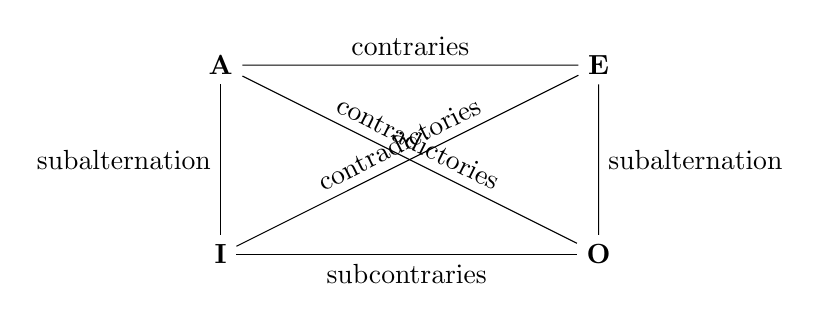
\begin{tikzpicture}[scale=1.2]
\node (A) at (0,2) {\(\mathbf{A}\)};
\node (E) at (4,2) {\(\mathbf{E}\)};
\node (I) at (0,0) {\(\mathbf{I}\)};
\node (O) at (4,0) {\(\mathbf{O}\)};

\draw (A) -- node[above]{contraries} (E);
\draw (I) -- node[below]{subcontraries} (O);

\draw (A) -- node[left]{subalternation} (I);
\draw (E) -- node[right]{subalternation} (O);

\draw (A) -- node[sloped,above]{contradictories} (O);
\draw (E) -- node[sloped,above]{contradictories} (I);
\end{tikzpicture}
\end{center}

The contradictory pairs are:

\[
A \leftrightarrow O
\]

and

\[
E \leftrightarrow I.
\]

Contradictories cannot both be true and cannot both be false.

Contraries cannot both be true, though they may both be false.

Subcontraries may both be true, but within the traditional
Aristotelian framework they are not both false.

Finally, Aristotle treats each universal statement as entailing
its corresponding particular.

\begin{whiteboard}
\textbf{SQUARE OF OPPOSITION}

\[
\begin{array}{ccc}
A & \longleftrightarrow & E\\
\rotatebox{90}{$\Rightarrow$} & & \rotatebox{90}{$\Rightarrow$}\\
I & \longleftrightarrow & O
\end{array}
\]

\[
A \leftrightarrow O
\quad\text{contradictories}
\]

\[
E \leftrightarrow I
\quad\text{contradictories}
\]

\[
A \leftrightarrow E
\quad\text{contraries}
\]

\[
I \leftrightarrow O
\quad\text{subcontraries}
\]

\[
A\Rightarrow I,
\qquad
E\Rightarrow O
\]
\end{whiteboard}

These relations generate an important problem.

% ============================================================
\section{Existential Import}
% ============================================================

Why should

\[
\text{Every }S\text{ is }P
\]

entail

\[
\text{Some }S\text{ is }P?
\]

That inference is valid only if something is in fact an \(S\).

Aristotle's logic behaves as though the general terms under
consideration have application.

\begin{whiteboard}
\textbf{EXISTENTIAL IMPORT}

Aristotle's framework assumes
that general terms have application.

\[
\text{Every }S\text{ is }P
\]

\[
\therefore
\text{Some }S\text{ is }P
\]

requires:

\[
\exists S
\]
\end{whiteboard}

The Kneales point out that modern logic need not make this
assumption.

Consider:

\begin{center}
``No mathematician has squared the circle.''
\end{center}

Rewriting it mechanically as

\begin{center}
``No mathematician is a person who has squared the circle''
\end{center}

must not lead us to assume that there actually exists a person who
has squared the circle.

\begin{whiteboard}
\textbf{MODERN CAUTION}

\[
\text{No mathematician has squared the circle}
\]

does not imply:

\[
\exists x(\text{\(x\) has squared the circle})
\]

\boardtakeaway{Existence should be asserted explicitly when it matters.}
\end{whiteboard}

The traditional square therefore works most naturally under
Aristotle's tacit assumption that its general terms have
application.

% ============================================================
\section{Conversion}
% ============================================================

Before Aristotle develops syllogistic, he studies
\textbf{conversion}.

Conversion interchanges the subject and predicate terms.

Certain forms convert simply.

Universal negatives:

\[
\text{No }S\text{ is }P
\]

convert to

\[
\text{No }P\text{ is }S.
\]

Particular affirmatives:

\[
\text{Some }S\text{ is }P
\]

convert to

\[
\text{Some }P\text{ is }S.
\]

Universal affirmatives convert only partially within Aristotle's
system:

\[
\text{Every }S\text{ is }P
\]

allows

\[
\text{Some }P\text{ is }S,
\]

provided the relevant existential assumptions hold.

Particular negatives do not simply convert.

\begin{whiteboard}
\textbf{CONVERSION}

\[
E:
\quad
\text{No }S\text{ is }P
\leftrightarrow
\text{No }P\text{ is }S
\]

\[
I:
\quad
\text{Some }S\text{ is }P
\leftrightarrow
\text{Some }P\text{ is }S
\]

\[
A:
\quad
\text{Every }S\text{ is }P
\Rightarrow
\text{Some }P\text{ is }S
\]

\[
O:
\quad
\text{no simple conversion}
\]

\boardtakeaway{Conversion = interchange subject and predicate.}
\end{whiteboard}

Conversion will become one of Aristotle's principal tools for
showing that syllogisms in different figures are valid.

% ============================================================
\section{The Introduction of Variables}
% ============================================================

The \textit{Prior Analytics} introduces one of Aristotle's most
important technical innovations: the use of letters as
\textbf{term variables}.

Earlier logical generality had often been expressed through
examples.

For instance:

\[
\text{Every man is an animal.}
\]

\[
\text{Every Greek is a man.}
\]

\[
\therefore
\text{Every Greek is an animal.}
\]

But the logical subject matter is clearer if we abstract from
``Greek,'' ``man,'' and ``animal.''

\begin{whiteboard}
\textbf{FROM EXAMPLE TO FORM}

\[
\begin{array}{l}
\text{Every man is an animal.}\\
\text{Every Greek is a man.}\\
\hline
\therefore \text{Every Greek is an animal.}
\end{array}
\]

becomes:

\[
\begin{array}{l}
\text{Every }M\text{ is }L.\\
\text{Every }S\text{ is }M.\\
\hline
\therefore \text{Every }S\text{ is }L.
\end{array}
\]

\boardtakeaway{VARIABLES expose FORM.}
\end{whiteboard}

The Kneales describe this use of variables as an epoch-making
advance in logical technique.

The letters do not stand for particular individuals. They mark
places into which general terms can be substituted.

% ============================================================
% PART III
% ============================================================

\part*{III. The Syllogistic System}

% ============================================================
\section{What Is a Syllogism?}
% ============================================================

At the beginning of the \textit{Prior Analytics}, Aristotle gives a
very broad definition of syllogism.

A syllogism is discourse in which, certain propositions having
been laid down, something different follows from them
\textbf{of necessity}.

In the \textit{Topics}, ``syllogism'' could therefore have a wide
meaning.

But Aristotle's detailed theory in the \textit{Prior Analytics}
becomes much narrower.

The characteristic categorical syllogism contains:

\begin{itemize}
    \item two premisses;
    \item three general terms;
    \item a conclusion;
    \item a middle term connecting the other two terms.
\end{itemize}

\begin{whiteboard}
\textbf{SYLLOGISM}

\[
\begin{array}{c}
\text{premiss}\\
\text{premiss}\\
\hline
\text{conclusion}
\end{array}
\]

\[
\boxed{\text{The conclusion follows OF NECESSITY.}}
\]

\vspace{0.5em}

Three terms:

\[
L=\text{major},
\qquad
S=\text{minor},
\qquad
M=\text{middle}
\]

\[
\boxed{
M\text{ occurs in both premisses but not in the conclusion.}
}
\]
\end{whiteboard}

In our notation, \(L\) is the predicate term of the conclusion,
\(S\) its subject term, and \(M\) the middle term.

This is a convenient later convention, not Aristotle's original
lettering.

% ============================================================
\section{From Plato's Division to Aristotle's Syllogism}
% ============================================================

Aristotle criticizes Plato's method of division as a method of
proof.

Suppose we divide animals into mortal and immortal animals, and
then place humans under the mortal branch.

That procedure may classify humans as mortal animals, but if the
classification is simply assumed in the division, it does not prove
that humans are mortal.

Division therefore risks begging the very point that requires
proof.

\begin{whiteboard}
\textbf{PLATO VS. ARISTOTLE}

\[
\begin{array}{rcl}
\text{Division}
&\rightarrow&
\text{classification}
\\[0.4em]
\text{Syllogism}
&\rightarrow&
\text{proof}
\end{array}
\]

\vspace{0.5em}

\[
L\text{ applies to }M
\]

\[
M\text{ applies to }S
\]

\[
\therefore
L\text{ applies to }S
\]
\end{whiteboard}

Although Aristotle rejects division as proof, the Kneales suggest
that the classificatory chain inherited from Plato helped shape
his conception of the syllogism.

% ============================================================
\section{The Three Figures}
% ============================================================

Aristotle distinguishes three figures according to the position of
the middle term.

Using our standardized notation:

\subsection{First Figure}

\[
\begin{array}{l}
M-L\\
S-M\\
\hline
S-L
\end{array}
\]

The middle term is subject in one premiss and predicate in the
other.

\subsection{Second Figure}

\[
\begin{array}{l}
L-M\\
S-M\\
\hline
S-L
\end{array}
\]

The middle term is predicate in both premisses.

\subsection{Third Figure}

\[
\begin{array}{l}
M-L\\
M-S\\
\hline
S-L
\end{array}
\]

The middle term is subject in both premisses.

\begin{whiteboard}
\textbf{THE THREE FIGURES}

\[
\begin{array}{c@{\qquad}c@{\qquad}c}
\textbf{1} & \textbf{2} & \textbf{3}\\[0.4em]
M-L & L-M & M-L\\
S-M & S-M & M-S\\
\hline
S-L & S-L & S-L
\end{array}
\]

\boardtakeaway{The position of the MIDDLE TERM determines the figure.}
\end{whiteboard}

Aristotle recognizes fourteen valid moods distributed across
these figures.

% ============================================================
\section{The Four First-Figure Moods}
% ============================================================

The medieval names for the moods were introduced later.

Nevertheless, they remain convenient labels.

The four fundamental first-figure moods are:

\subsection{Barbara}

\[
\begin{array}{l}
\text{Every }M\text{ is }L.\\
\text{Every }S\text{ is }M.\\
\hline
\therefore\text{Every }S\text{ is }L.
\end{array}
\]

\subsection{Celarent}

\[
\begin{array}{l}
\text{No }M\text{ is }L.\\
\text{Every }S\text{ is }M.\\
\hline
\therefore\text{No }S\text{ is }L.
\end{array}
\]

\begin{whiteboard}
\textbf{FIRST FIGURE I}

\[
\textbf{BARBARA}
\]

\[
\begin{array}{l}
\text{Every }M\text{ is }L.\\
\text{Every }S\text{ is }M.\\
\hline
\therefore\text{Every }S\text{ is }L.
\end{array}
\]

\vspace{0.5em}

\[
\textbf{CELARENT}
\]

\[
\begin{array}{l}
\text{No }M\text{ is }L.\\
\text{Every }S\text{ is }M.\\
\hline
\therefore\text{No }S\text{ is }L.
\end{array}
\]

\textit{Copy, then erase.}
\end{whiteboard}

\subsection{Darii}

\[
\begin{array}{l}
\text{Every }M\text{ is }L.\\
\text{Some }S\text{ is }M.\\
\hline
\therefore\text{Some }S\text{ is }L.
\end{array}
\]

\subsection{Ferio}

\[
\begin{array}{l}
\text{No }M\text{ is }L.\\
\text{Some }S\text{ is }M.\\
\hline
\therefore\text{Some }S\text{ is not }L.
\end{array}
\]

\begin{whiteboard}
\textbf{FIRST FIGURE II}

\[
\textbf{DARII}
\]

\[
\begin{array}{l}
\text{Every }M\text{ is }L.\\
\text{Some }S\text{ is }M.\\
\hline
\therefore\text{Some }S\text{ is }L.
\end{array}
\]

\vspace{0.5em}

\[
\textbf{FERIO}
\]

\[
\begin{array}{l}
\text{No }M\text{ is }L.\\
\text{Some }S\text{ is }M.\\
\hline
\therefore\text{Some }S\text{ is not }L.
\end{array}
\]

\[
\boxed{\text{Aristotle recognizes fourteen valid moods in all.}}
\]
\end{whiteboard}

% ============================================================
\section{Reference: Aristotle's Fourteen Valid Moods}
% ============================================================

The following table is included for reference.
Students need not memorize the medieval names at this stage.

\begin{center}
\small
\begin{tabularx}{\textwidth}{c l X}
\toprule
\textbf{Figure} & \textbf{Mood} & \textbf{Form}\\
\midrule
1 & Barbara &
Every \(M\) is \(L\); Every \(S\) is \(M\); therefore Every \(S\) is \(L\).\\

1 & Celarent &
No \(M\) is \(L\); Every \(S\) is \(M\); therefore No \(S\) is \(L\).\\

1 & Darii &
Every \(M\) is \(L\); Some \(S\) is \(M\); therefore Some \(S\) is \(L\).\\

1 & Ferio &
No \(M\) is \(L\); Some \(S\) is \(M\); therefore Some \(S\) is not \(L\).\\
\midrule

2 & Cesare &
No \(L\) is \(M\); Every \(S\) is \(M\); therefore No \(S\) is \(L\).\\

2 & Camestres &
Every \(L\) is \(M\); No \(S\) is \(M\); therefore No \(S\) is \(L\).\\

2 & Festino &
No \(L\) is \(M\); Some \(S\) is \(M\); therefore Some \(S\) is not \(L\).\\

2 & Baroco &
Every \(L\) is \(M\); Some \(S\) is not \(M\); therefore Some \(S\) is not \(L\).\\
\midrule

3 & Darapti &
Every \(M\) is \(L\); Every \(M\) is \(S\); therefore Some \(S\) is \(L\).\\

3 & Felapton &
No \(M\) is \(L\); Every \(M\) is \(S\); therefore Some \(S\) is not \(L\).\\

3 & Disamis &
Some \(M\) is \(L\); Every \(M\) is \(S\); therefore Some \(S\) is \(L\).\\

3 & Datisi &
Every \(M\) is \(L\); Some \(M\) is \(S\); therefore Some \(S\) is \(L\).\\

3 & Bocardo &
Some \(M\) is not \(L\); Every \(M\) is \(S\); therefore Some \(S\) is not \(L\).\\

3 & Ferison &
No \(M\) is \(L\); Some \(M\) is \(S\); therefore Some \(S\) is not \(L\).\\
\bottomrule
\end{tabularx}
\end{center}

Darapti and Felapton depend upon Aristotle's assumption of
existential import. Without an assumption that there actually are
\(M\)'s, their particular conclusions do not follow from their two
universal premisses.

% ============================================================
\section{Worked Example: Barbara}
% ============================================================

Consider:

\[
\text{Every mammal is an animal.}
\]

\[
\text{Every dog is a mammal.}
\]

Therefore:

\[
\text{Every dog is an animal.}
\]

\begin{whiteboard}
\textbf{BARBARA: CONCRETE FORM}

\[
\begin{array}{l}
\text{Every mammal is an animal.}\\
\text{Every dog is a mammal.}\\
\hline
\therefore \text{Every dog is an animal.}
\end{array}
\]
\end{whiteboard}

Now replace the particular content with variables.

\begin{whiteboard}
\textbf{BARBARA: ABSTRACT FORM}

\[
\begin{array}{l}
\text{Every }M\text{ is }L.\\
\text{Every }S\text{ is }M.\\
\hline
\therefore \text{Every }S\text{ is }L.
\end{array}
\]

\boardtakeaway{CONTENT changes; FORM remains.}
\end{whiteboard}

The variables reveal precisely what makes the inference
independent of its subject matter.

% ============================================================
\section{Why the First Figure Is ``Perfect''}
% ============================================================

Aristotle calls first-figure syllogisms \textbf{perfect}.

The likely reason is that their necessity becomes evident from the
arrangement of terms without requiring supplementary
transformations.

Barbara can be visualized pedagogically as:

\[
S\subseteq M
\]

and

\[
M\subseteq L,
\]

hence:

\[
S\subseteq L.
\]

This class notation is a modern explanatory device, not
Aristotle's symbolism.

\begin{whiteboard}
\textbf{WHY FIGURE 1 IS ``PERFECT''}

\[
S\subseteq M
\]

\[
M\subseteq L
\]

\[
\therefore S\subseteq L
\]

\boardtakeaway{The transitivity of the term connexion is visible.}
\end{whiteboard}

The other figures require additional work to show that their
conclusions follow.

% ============================================================
\section{The Special Character of the Three Figures}
% ============================================================

The Kneales summarize the figures in useful conceptual terms.

In the \textbf{first figure}, the reasoner establishes a conclusion
by showing that a sufficient condition is fulfilled.

In the \textbf{second figure}, the conclusion must be negative.
The argument shows that a necessary condition is not fulfilled.

In the \textbf{third figure}, the conclusion must be particular.
The argument proceeds through instances.

\begin{whiteboard}
\textbf{THREE FIGURES: LOGICAL CHARACTER}

\[
\begin{array}{rl}
\textbf{Figure 1:} & \text{sufficient condition fulfilled}\\[0.4em]
\textbf{Figure 2:} & \text{necessary condition fails}\\[0.4em]
\textbf{Figure 3:} & \text{instances establish a particular}
\end{array}
\]
\end{whiteboard}

This interpretation also helps explain why existential assumptions
are particularly important in the third figure.

% ============================================================
\section{How Aristotle Rejects Invalid Forms}
% ============================================================

Aristotle does not merely list valid moods.

He also considers pairs of premiss forms that fail to determine
any necessary conclusion.

One important technique is what the Kneales call
\textbf{rejection by contrasted instances}.

Suppose the premisses have the form:

\[
\text{Every }M\text{ is }L
\]

and

\[
\text{No }S\text{ is }M.
\]

Does anything follow about the relation between \(S\) and \(L\)?

Consider first:

\[
M=\text{man},
\quad
L=\text{animal},
\quad
S=\text{horse}.
\]

The premisses are true:

\[
\text{Every man is an animal}
\]

and

\[
\text{No horse is a man}.
\]

Yet:

\[
\text{Every horse is an animal}.
\]

Now change only \(S\):

\[
S=\text{stone}.
\]

Again the premisses are true:

\[
\text{Every man is an animal}
\]

and

\[
\text{No stone is a man}.
\]

But:

\[
\text{No stone is an animal}.
\]

The same premiss form is therefore compatible with opposite
relations between \(S\) and \(L\).

\begin{whiteboard}
\textbf{CONTRASTED INSTANCES}

Premiss form:

\[
\text{Every }M\text{ is }L
\]

\[
\text{No }S\text{ is }M
\]

Case 1:

\[
M=\text{man},\quad L=\text{animal},\quad S=\text{horse}
\]

\[
\text{Every horse is an animal}
\]

Case 2:

\[
M=\text{man},\quad L=\text{animal},\quad S=\text{stone}
\]

\[
\text{No stone is an animal}
\]
\end{whiteboard}

Therefore the original premiss structure determines neither an
affirmative nor a negative conclusion.

\begin{whiteboard}
\[
\boxed{\text{NO NECESSARY CONCLUSION}}
\]

\boardtakeaway{Counterexamples can refute a proposed argument form.}
\end{whiteboard}

This is an important early use of counterexample-style reasoning
in formal logic.

% ============================================================
\section{Reduction}
% ============================================================

Aristotle's fourteen valid moods are not merely a catalogue.

He organizes the system through the doctrine of
\textbf{reduction}.

Syllogisms in the second and third figures are validated by
transforming them into first-figure syllogisms.

\begin{whiteboard}
\textbf{REDUCTION}

\[
\begin{array}{c}
\text{Figure 2 or Figure 3}\\
\downarrow\\
\text{conversion / transformation}\\
\downarrow\\
\text{Figure 1}
\end{array}
\]

\boardtakeaway{``Imperfect'' moods are validated through ``perfect'' moods.}
\end{whiteboard}

For most moods, conversion is enough.

Two moods, however, require an indirect procedure:

\begin{itemize}
    \item Baroco;
    \item Bocardo.
\end{itemize}

For these Aristotle uses what later came to be called
\textit{reduction per impossibile}.

% ============================================================
\section{Worked Example: Indirect Reduction}
% ============================================================

Consider the Baroco form:

\[
\text{Every }L\text{ is }M.
\]

\[
\text{Some }S\text{ is not }M.
\]

Therefore:

\[
\text{Some }S\text{ is not }L.
\]

\newpage

\begin{whiteboard}
\textbf{INDIRECT REDUCTION: PACKET 1}

Given:

\[
\text{Every }L\text{ is }M
\]

\[
\text{Some }S\text{ is not }M
\]

Want:

\[
\text{Some }S\text{ is not }L
\]

Assume the contradictory:

\[
\text{Every }S\text{ is }L
\]

\textit{Copy, then erase.}
\end{whiteboard}

Now combine:

\[
\text{Every }L\text{ is }M
\]

with

\[
\text{Every }S\text{ is }L.
\]

Barbara gives:

\[
\text{Every }S\text{ is }M.
\]

But the original premiss says:

\[
\text{Some }S\text{ is not }M.
\]

Contradiction.

Therefore the denial of the original conclusion cannot stand.

\newpage

\begin{whiteboard}
\textbf{INDIRECT REDUCTION: PACKET 2}

\[
\text{Every }L\text{ is }M
\]

\[
\text{Every }S\text{ is }L
\]

\[
\therefore
\text{Every }S\text{ is }M
\]

But:

\[
\text{Some }S\text{ is not }M
\]

Therefore:

\[
\bot
\]

and hence:

\[
\boxed{\text{Some }S\text{ is not }L}
\]

\[
\textbf{REDUCTION PER IMPOSSIBILE}
\]
\end{whiteboard}

The procedure connects Aristotle's formal system directly with
the older Greek tradition of reductio.

% ============================================================
\section{Ecthesis}
% ============================================================

Aristotle also sometimes uses a method called
\textbf{ecthesis}, literally a ``setting out.''

The basic procedure is to introduce an appropriate instance in
order to reason about a general relation.

\begin{whiteboard}
\textbf{ECTHESIS}

\[
\begin{array}{c}
\text{general claim}\\
\downarrow\\
\text{set out an appropriate instance}\\
\downarrow\\
\text{reason from that instance}
\end{array}
\]
\end{whiteboard}

Ancient and modern scholars have disputed whether Aristotle's
introduced item should always be understood as an individual or
sometimes as a subclass.

For our purposes, the important point is simply that ecthesis is
another technique by which Aristotle validates logical
transformations.

% ============================================================
\section{Aristotle's System Is Not a Modern Axiomatic System}
% ============================================================

Modern textbooks often present Barbara like this:

\[
\begin{array}{l}
\text{Every }M\text{ is }L.\\
\text{Every }S\text{ is }M.\\
\hline
\therefore\text{Every }S\text{ is }L.
\end{array}
\]

Aristotle's own characteristic formulation is instead a
conditional principle:

\[
\text{If every }M\text{ is }L
\text{ and every }S\text{ is }M,
\]

\[
\text{then necessarily every }S\text{ is }L.
\]

Later antiquity increasingly presented the theory through
inference schemata.

The difference should not be exaggerated, since Aristotle uses
his conditional principles much as rules of inference.

But historically we should not simply reconstruct his theory as
though it were already a modern formal calculus.

\begin{whiteboard}
\textbf{ARISTOTLE'S PRESENTATION}

\[
\text{If }P_1\text{ and }P_2,
\text{ then necessarily }C.
\]

Later presentation:

\[
\begin{array}{c}
P_1\\
P_2\\
\hline
C
\end{array}
\]

\[
\boxed{
\text{Systematic? YES}
\qquad
\text{Modern axiomatic calculus? NO}
}
\]
\end{whiteboard}

Later logicians, most notably Jan Lukasiewicz, successfully
reconstructed Aristotelian syllogistic as an axiomatic deductive
system.

That reconstruction is logically interesting but should not be
confused with Aristotle's own conception of his work.

% ============================================================
% PART IV
% ============================================================

\part*{IV. Beyond Pure Assertoric Syllogistic}

% ============================================================
\section{Modal Logic}
% ============================================================

Aristotle does not limit himself to ordinary, or
\textbf{assertoric}, propositions.

He also attempts a theory of modal propositions and modal
syllogisms.

A modal proposition contains such notions as necessity or
possibility.

The three broad kinds relevant to Aristotle's treatment are:

\begin{itemize}
    \item assertoric;
    \item apodeictic;
    \item problematic.
\end{itemize}

\begin{whiteboard}
\textbf{MODAL STATEMENTS}

\[
\begin{array}{rl}
\textbf{Assertoric:} & P\\[0.4em]
\textbf{Apodeictic:} & \text{necessarily }P\\[0.4em]
\textbf{Problematic:} & \text{possibly / contingently }P
\end{array}
\]

\boardtakeaway{Modal logic asks how modality changes inference.}
\end{whiteboard}

The Kneales judge Aristotle's modal syllogistic to be much less
successful than his assertoric syllogistic.

The theory is complicated, lacks sufficiently clear symbolism,
and is developed without a prior systematic logic of propositions.

Nevertheless, Aristotle's decision to treat modality logically is
itself a major achievement.

% ============================================================
\section{Necessity, Possibility, and Contingency}
% ============================================================

The Kneales distinguish two notions that Aristotle expresses with
closely related terminology.

In the broad sense:

\[
\text{possible }P
\]

means:

\[
\text{not impossible }P.
\]

But Aristotle's stricter problematic notion is better translated
by the Kneales as \textbf{contingent}.

A proposition is contingent when it is possible but not
necessary.

Thus:

\[
\text{Contingent }P
=
\text{Possible }P
\land
\neg\text{Necessary }P.
\]

\begin{whiteboard}
\textbf{MODAL RELATIONS}

\[
\text{Necessary }P
\Rightarrow
\text{Possible }P
\]

\[
\text{Impossible }P
=
\text{Necessary }\neg P
\]

\[
\text{Possible }P
=
\neg\text{Necessary }\neg P
\]

\[
\boxed{
\text{Contingent }P
=
\text{Possible }P
\land
\neg\text{Necessary }P
}
\]
\end{whiteboard}

One difficulty in Aristotle's modal syllogistic is precisely that
contingency is already logically complex.

% ============================================================
\section{The Modal Square}
% ============================================================

The modal notions can be arranged by analogy with the ordinary
square of opposition.

\begin{center}
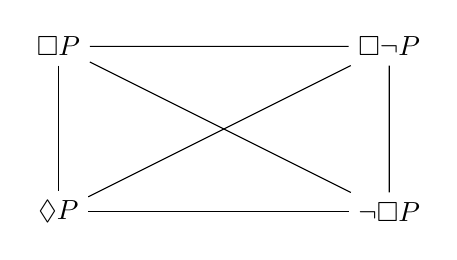
\begin{tikzpicture}[scale=1.05]
\node (N) at (0,2) {\(\Box P\)};
\node (I) at (4,2) {\(\Box\neg P\)};
\node (P) at (0,0) {\(\Diamond P\)};
\node (NN) at (4,0) {\(\neg\Box P\)};

\draw (N) -- (I);
\draw (P) -- (NN);
\draw (N) -- (P);
\draw (I) -- (NN);
\draw (N) -- (NN);
\draw (I) -- (P);
\end{tikzpicture}
\end{center}

Here:

\[
\Box P
\]

means that \(P\) is necessary,

and:

\[
\Diamond P
\]

means that \(P\) is possible.

Contingency is represented by the conjunction:

\[
\Diamond P\land\neg\Box P.
\]

\begin{whiteboard}
\textbf{MODAL SQUARE}

\[
\begin{array}{ccc}
\text{Necessary }P
&&
\text{Impossible }P
\\[1em]
\text{Possible }P
&&
\text{Not-necessary }P
\end{array}
\]

\[
\boxed{
\text{Contingent }P
=
\text{Possible }P
+
\text{Not-necessary }P
}
\]
\end{whiteboard}

% ============================================================
\section{Separately Possible Does Not Mean Jointly Possible}
% ============================================================

One source of difficulty in modal reasoning is the assumption that
two things that are separately possible must also be possible
together.

But:

\[
\Diamond P
\]

and

\[
\Diamond Q
\]

do not in general entail:

\[
\Diamond(P\land Q).
\]

\begin{whiteboard}
\textbf{MODAL CAUTION}

\[
\Diamond P
\]

\[
\Diamond Q
\]

does \textbf{not} guarantee:

\[
\Diamond(P\land Q)
\]

\boardtakeaway{SEPARATELY POSSIBLE $\neq$ JOINTLY POSSIBLE}
\end{whiteboard}

This kind of problem helps explain why problematic syllogistic
cannot simply be obtained by inserting modal words into ordinary
syllogisms.

% ============================================================
\section{The Scope of Modality}
% ============================================================

Another major difficulty concerns where the modal qualification
belongs.

Compare:

\[
\Box(\text{Every }B\text{ is }A)
\]

with:

\[
\text{Every }B\text{ is necessarily-}A.
\]

These are not automatically equivalent.

The modal qualification should not simply be treated as though it
were an ordinary component of the predicate.

\begin{whiteboard}
\textbf{SCOPE MATTERS}

Correct logical structure:

\[
\Box(\text{Every }B\text{ is }A)
\]

Do not automatically rewrite as:

\[
\text{Every }B\text{ is }\Box A
\]

\boardtakeaway{The modality qualifies the proposition as a whole.}
\end{whiteboard}

The Kneales use this distinction to diagnose some of Aristotle's
unsuccessful modal syllogisms.

% ============================================================
\section{Why Modality Belongs in Logic}
% ============================================================

Aristotle's technical modal theory is imperfect.

But the Kneales argue that Aristotle was entirely right to regard
modality as part of logic.

There are two reasons.

First, distinctions between:

\[
\text{true},
\quad
\text{necessary},
\quad
\text{false},
\quad
\text{impossible}
\]

apply across subject matters.

Second, the very notion of validity is naturally expressed in
modal language.

An argument is valid when it is \textbf{impossible} for its
premisses to be true while its conclusion is false.

\begin{whiteboard}
\textbf{VALIDITY}

A valid argument makes this impossible:

\[
\text{premisses true}
\land
\text{conclusion false}
\]

Symbolically:

\[
\boxed{
\neg\Diamond
(\text{Premisses true}\land\text{Conclusion false})
}
\]

\boardtakeaway{Logic itself uses modality.}
\end{whiteboard}

Aristotle therefore deserves credit for initiating logical inquiry
into modality even where the resulting details are defective.

% ============================================================
\section{Non-Syllogistic Logic in the Analytics}
% ============================================================

The \textit{Prior Analytics} contains logical principles that do
not belong to categorical syllogistic.

The Kneales identify two especially important principles that can
be expressed in modern terminology as
\textbf{contraposition} and
\textbf{transitivity of entailment}.

% ============================================================
\subsection{Contraposition}
% ============================================================

If \(P\) entails \(Q\), then the falsity of \(Q\) entails the
falsity of \(P\).

\[
P\Rightarrow Q
\]

therefore:

\[
\neg Q\Rightarrow\neg P.
\]

\begin{whiteboard}
\textbf{CONTRAPOSITION}

\[
P\Rightarrow Q
\]

\[
\therefore
\neg Q\Rightarrow\neg P
\]
\end{whiteboard}

% ============================================================
\subsection{Transitivity}
% ============================================================

If \(P\) entails \(Q\), and \(Q\) entails \(R\), then \(P\)
entails \(R\).

\[
P\Rightarrow Q
\]

\[
Q\Rightarrow R
\]

therefore:

\[
P\Rightarrow R.
\]

\begin{whiteboard}
\textbf{TRANSITIVITY OF ENTAILMENT}

\[
P\Rightarrow Q
\]

\[
Q\Rightarrow R
\]

\[
\therefore
P\Rightarrow R
\]

\boardtakeaway{These principles concern propositions, not merely relations among terms.}
\end{whiteboard}

These passages are important because they show that Aristotle's
logical insights extend beyond the formal boundaries of his
syllogistic system.

% ============================================================
\section{``Either Way, We Must Philosophize''}
% ============================================================

The Kneales also preserve an argument from Aristotle's early
\textit{Protrepticus}.

Its idea is:

\begin{itemize}
    \item either we ought to philosophize or we ought not;
    \item if we ought, then we ought to philosophize;
    \item if we ought not, philosophical reasoning is still needed
    to justify that claim;
    \item therefore, in either case, we must philosophize.
\end{itemize}

Abstractly, the form is:

\[
P\lor\neg P
\]

\[
P\Rightarrow Q
\]

\[
\neg P\Rightarrow Q
\]

therefore:

\[
Q.
\]

\begin{whiteboard}
\textbf{EITHER WAY}

\[
P\lor\neg P
\]

\[
P\Rightarrow Q
\]

\[
\neg P\Rightarrow Q
\]

\[
\therefore Q
\]

Application:

\[
\boxed{\text{Either way, we must philosophize.}}
\]
\end{whiteboard}

This kind of reasoning does not fit naturally into categorical
syllogistic.

It points toward a logic whose units are whole propositions.

% ============================================================
\section{Reasoning From Hypothesis}
% ============================================================

Aristotle recognizes arguments ``from hypothesis,'' but he does
not build a systematic logic of conditionals comparable to his
theory of syllogisms.

Two forms that later become fundamental are:

\[
\text{If }P\text{ then }Q;
\quad
P;
\quad
\therefore Q
\]

and:

\[
\text{If }P\text{ then }Q;
\quad
\neg Q;
\quad
\therefore\neg P.
\]

\newpage

\begin{whiteboard}
\textbf{CONDITIONAL ARGUMENT FORMS}

\[
\begin{array}{c}
P\rightarrow Q\\
P\\
\hline
Q
\end{array}
\]

and

\[
\begin{array}{c}
P\rightarrow Q\\
\neg Q\\
\hline
\neg P
\end{array}
\]
\end{whiteboard}

The second is the form underlying many reductio arguments.

The Kneales' criticism is not that Aristotle never uses such
reasoning.

He plainly does.

The limitation is that he does not isolate and systematize the
logical distinction between these forms in the way later
propositional logicians will.

% ============================================================
\section{Theophrastus}
% ============================================================

Aristotle's logical project continued immediately within his own
school.

Theophrastus succeeded Aristotle as head of the Lyceum.

His logical works no longer survive intact, so our knowledge
depends heavily on later reports.

Nevertheless, he appears to have extended Aristotle's work in
several directions.

\begin{whiteboard}
\textbf{THEOPHRASTUS}

Extends Aristotle in:

\[
\begin{array}{ll}
1. & \text{syllogistic}\\
2. & \text{modal logic}\\
3. & \text{hypothetical logic}
\end{array}
\]

\[
\text{Aristotle}
\longrightarrow
\text{Theophrastus}
\longrightarrow
\text{later tradition}
\]
\end{whiteboard}

% ============================================================
\section{Indirect Moods and the Later Fourth Figure}
% ============================================================

Theophrastus is reported to have recognized additional indirect
forms associated with Aristotle's first figure.

Later tradition reorganized such forms as a
\textbf{fourth figure}.

Its characteristic pattern may be represented:

\[
\begin{array}{l}
L-M\\
M-S\\
\hline
S-L
\end{array}
\]

\begin{whiteboard}
\textbf{LATER ``FOURTH FIGURE''}

\[
\begin{array}{l}
L-M\\
M-S\\
\hline
S-L
\end{array}
\]

\[
\begin{array}{rcl}
\text{Aristotle} &:& 3\text{ figures}\\
\text{later tradition} &:& 4\text{ figures}
\end{array}
\]

\boardtakeaway{Whether this is a separate figure depends upon how ``figure'' is defined.}
\end{whiteboard}

The point is historically interesting but less important than
Theophrastus' contribution to hypothetical reasoning.

% ============================================================
\section{Theophrastus and Modal Logic}
% ============================================================

Aristotle's immediate successors already recognized difficulties
in his modal syllogistic.

Theophrastus appears to have revised parts of the system.

Because the ancient evidence is fragmentary, we should avoid
pretending that we possess a complete reconstruction.

The important historical point is the speed with which
formalization generated criticism and revision.

\begin{whiteboard}
\textbf{MODAL SYLLOGISTIC}

\[
\begin{array}{c}
\text{Aristotle}\\
\downarrow\\
\text{technical difficulties}\\
\downarrow\\
\text{Theophrastus revises}
\end{array}
\]

\boardtakeaway{Formalization exposed problems that informal reasoning had hidden.}
\end{whiteboard}

% ============================================================
\section{Hypothetical Reasoning}
% ============================================================

In the ancient Peripatetic tradition, the word ``hypothetical''
has a broader range than our modern word ``conditional.''

It can include reasoning involving complex premisses such as:

\[
P\rightarrow Q,
\]

\[
P\lor Q,
\]

and

\[
\neg(P\land Q).
\]

\begin{whiteboard}
\textbf{``HYPOTHETICAL''}

In this tradition:

\[
\text{hypothetical argument}
\approx
\text{argument with a complex premiss}
\]

Examples:

\[
P\rightarrow Q
\]

\[
P\lor Q
\]

\[
\neg(P\land Q)
\]

\boardtakeaway{This points beyond categorical syllogistic.}
\end{whiteboard}

The evidence does not allow us to reconstruct a complete
Aristotelian hypothetical logic, but the material becomes
increasingly important in Aristotle's school.

% ============================================================
\section{A Conditional Argument}
% ============================================================

A reported example has the form:

\begin{center}
If the soul always moves, the soul is immortal.
\end{center}

\begin{center}
The soul always moves.
\end{center}

Therefore:

\begin{center}
The soul is immortal.
\end{center}

The logical pattern is:

\[
P\rightarrow Q
\]

\[
P
\]

\[
\therefore Q.
\]

\begin{whiteboard}
\textbf{CONDITIONAL INFERENCE}

\[
\begin{array}{c}
P\rightarrow Q\\
P\\
\hline
Q
\end{array}
\]

\[
\text{conditional premiss}
+
\text{additional premiss}
\rightarrow
\text{conclusion}
\]
\end{whiteboard}

We should not infer from this that Aristotle or Theophrastus had
already produced the mature Stoic propositional logic.

It does show that the Peripatetic tradition was developing logical
patterns not reducible to ordinary term syllogisms.

% ============================================================
\section{Theophrastus and Inference Schemata}
% ============================================================

Later testimony credits Theophrastus with systematic treatment
of what were called totally hypothetical syllogisms.

One form is:

\[
P\rightarrow Q
\]

\[
Q\rightarrow R
\]

therefore:

\[
P\rightarrow R.
\]

\begin{whiteboard}
\textbf{THEOPHRASTUS}

\[
P\rightarrow Q
\]

\[
Q\rightarrow R
\]

\[
\therefore
P\rightarrow R
\]

\[
\boxed{\text{transitivity of implication}}
\]
\end{whiteboard}

The Kneales emphasize another historically interesting point.

Aristotle usually states the logical principle corresponding to a
mood as a conditional sentence:

\[
\text{If the premisses hold, the conclusion necessarily follows.}
\]

Theophrastus appears to have presented hypothetical reasoning
through something much closer to an explicit
\textbf{inference schema}.

\begin{whiteboard}
\textbf{FROM TERM PATTERNS TO PROPOSITION PATTERNS}

Aristotelian emphasis:

\[
S,M,L
\]

Theophrastean hypothetical form:

\[
P,Q,R
\]

\[
\boxed{\text{Whole propositions become the units of the pattern.}}
\]
\end{whiteboard}

This development points directly toward the Megarian and Stoic
tradition.

% ============================================================
\section{Prosleptic Reasoning}
% ============================================================

Theophrastus is also associated with
\textbf{prosleptic syllogisms}.

The important conceptual feature is that such reasoning can
generalize over kinds or predicates themselves rather than merely
over individual things.

A source example can be represented approximately as follows:

\begin{itemize}
    \item substance is predicable of whatever is universally
    predicable of man;
    \item animal is universally predicable of man;
    \item therefore substance is predicable of animal.
\end{itemize}

The abstract structure is more important than the terminology.

\begin{whiteboard}
\textbf{PROSLEPTIC REASONING}

Ordinary syllogistic:

\[
\text{generalizes over individuals}
\]

Prosleptic pattern:

\[
\text{generalizes over kinds / predicates}
\]

Abstractly:

\[
\begin{array}{c}
\text{Whatever satisfies }C\text{ has }A\\
B\text{ satisfies }C\\
\hline
\therefore B\text{ has }A
\end{array}
\]
\end{whiteboard}

The Kneales compare aspects of this with later ideas of
substitution and detachment.

% ============================================================
\section{What Aristotle Achieved}
% ============================================================

Aristotle's achievement can now be stated more precisely.

He provides:

\begin{itemize}
    \item an explicit classification of general propositions;
    \item a systematic account of opposition;
    \item the use of logical variables;
    \item a formal theory of categorical syllogisms;
    \item a classification into figures and moods;
    \item techniques for rejecting invalid forms;
    \item conversion;
    \item reduction of imperfect to perfect syllogisms;
    \item indirect reduction;
    \item an attempt at modal logic;
    \item principles of entailment beyond syllogistic.
\end{itemize}

\begin{whiteboard}
\textbf{ARISTOTLE'S ACHIEVEMENT}

\[
\begin{array}{ll}
\checkmark & \text{quantified proposition forms}\\
\checkmark & \text{variables}\\
\checkmark & \text{systematic syllogistic}\\
\checkmark & \text{valid / invalid forms}\\
\checkmark & \text{reduction}\\
\checkmark & \text{modal inquiry}\\
\checkmark & \text{general entailment principles}
\end{array}
\]
\end{whiteboard}

These discoveries justify Aristotle's extraordinary position in
the history of logic.

% ============================================================
\section{The Limits of Aristotle's Framework}
% ============================================================

The same chapter also reveals important limitations.

Aristotle's conception of the proposition is dominated by the
subject--predicate structure.

His system does not sharply enough distinguish singular from
general propositions.

It tacitly assumes application for general terms in places where
modern logic makes existence explicit.

Relations receive only scattered treatment.

Complex propositions are not systematically developed into a
logic of propositions.

And the modal syllogistic contains serious technical problems.

\begin{whiteboard}
\textbf{LIMITS}

\[
\begin{array}{ll}
\times & \text{subject--predicate dominance}\\
\times & \text{singular/general distinction blurred}\\
\times & \text{existential assumptions}\\
\times & \text{relations underdeveloped}\\
\times & \text{no complete propositional logic}\\
\times & \text{problematic modal system}
\end{array}
\]

\vspace{0.5em}

\[
\boxed{\text{Yet this is the first systematic formal logic.}}
\]
\end{whiteboard}

The limitations do not diminish the achievement.

They explain the direction in which subsequent logical
development had to proceed.

% ============================================================
\section{Two Directions After Aristotle}
% ============================================================

By the end of the chapter, two lines of development have become
visible.

The first is Aristotle's great achievement:

\[
\text{categorical syllogistic}.
\]

Its primary objects are relations among general terms.

The second emerges through material Aristotle does not fully
systematize and through the work of Theophrastus:

\[
\text{hypothetical and propositional reasoning}.
\]

Its primary objects increasingly become relations among whole
propositions.

\begin{whiteboard}
\textbf{TWO DIRECTIONS}

\[
\begin{array}{c}
\textbf{ARISTOTLE}\\
\downarrow\\
\text{categorical syllogistic}\\
\text{relations among terms}
\end{array}
\]

\[
\begin{array}{c}
\textbf{THEOPHRASTUS}\\
\downarrow\\
\text{hypothetical developments}\\
\text{relations among propositions}\\
\downarrow\\
\textbf{MEGARIANS + STOICS}
\end{array}
\]
\end{whiteboard}

This gives us the transition to the next chapter.

% ============================================================
\section{Lecture Summary}
% ============================================================

Aristotle inherited a Greek tradition in which thinkers already
reasoned about demonstration, dialectic, fallacy, truth,
definition, and necessary connexion.

His achievement was to transform this material into a
systematic investigation of logical form.

The \textit{Categories} supplied a metaphysical and linguistic
framework centered on predication.

The \textit{Topics} contained logical theory still embedded in
dialectical practice.

The \textit{De Interpretatione} isolated forms of statement and
their oppositions.

The \textit{Prior Analytics} introduced variables and created the
first systematic theory of syllogistic inference.

Aristotle then attempted to extend formal logic to modality and
also stated principles of entailment that reached beyond the
limits of his categorical theory.

Theophrastus continued the project and pushed the Peripatetic
tradition toward increasingly explicit hypothetical reasoning.

\begin{whiteboard}
\textbf{CHAPTER II SUMMARY}

\[
\begin{array}{c}
\textit{Categories}\\
\downarrow\\
\text{predication}
\\[0.7em]
\textit{Topics}\\
\downarrow\\
\text{dialectical patterns}
\\[0.7em]
\textit{De Interpretatione}\\
\downarrow\\
A,E,I,O
\\[0.7em]
\textit{Prior Analytics}\\
\downarrow\\
\text{variables + syllogistic}
\\[0.7em]
\text{modal / non-syllogistic work}\\
\downarrow\\
\text{Theophrastus}
\end{array}
\]
\end{whiteboard}

\begin{whiteboard}
\textbf{FINAL TAKEAWAY}

\[
\boxed{
\begin{array}{c}
\text{Aristotle did not invent reasoning.}\\[0.3em]
\text{He invented a systematic formal theory}\\
\text{for studying important forms of reasoning.}
\end{array}
}
\]

\vspace{0.8em}

\[
\text{Next: The Megarians and the Stoics}
\]
\end{whiteboard}

\end{document}